\section{REBT and CT: Cognitive Behavior Approaches}

\begin{coloredlist}
    \item REBT and CT were devloped around th esame time, independently of each other.
    \item Therapists with backgrounds from either approach now call themselves cognitive-behavioral therapists.
    \item Both approaches consider mental health problems to stem (at least in part) from maladaptive thinking.
    \item Both address problematic thinking patterns and help clients develop healthier views about themselves, the world, and the future.
    \item \textit{Thoughts, emotions, and behaviors interact} significantly and have reciprocal cause-and-effect relationships.
\end{coloredlist}

\subsection{Albert Ellis' Rational Emotive Behavior Therapy (REBT)}

\begin{coloredlist}
    \item Originally trained as a psychoanalyst, Ellis developed REBT in the 1950s.
    \item He was frustrated with slow client process.
    \item Noticed that clients appeared to make progress when they \textit{changed how they thought} about themselves and their problems.
    \item Basic Assumption of REBT: People \textbf{contribute to their own psychological problems} and symptoms due to rigid and extreme beliefs they hold.
    \item Clients must learn to fully accept themselves.
\end{coloredlist}

\subsection{Aaron Beck's Cognitive Therapy (CT)}

\begin{coloredlist}
    \item Developed by Aaron Beck based on his research.
    \item CT is shown to effectively treat a wide range of mental health disorders.
    \item Posits that the cognitive triad causes the maintenance of depressive symptoms, regardless of initial cause (negative thoughts about oneself, the world, and the future).
\end{coloredlist}

\begin{coloredlist}
    \item \textbf{d}
\end{coloredlist}

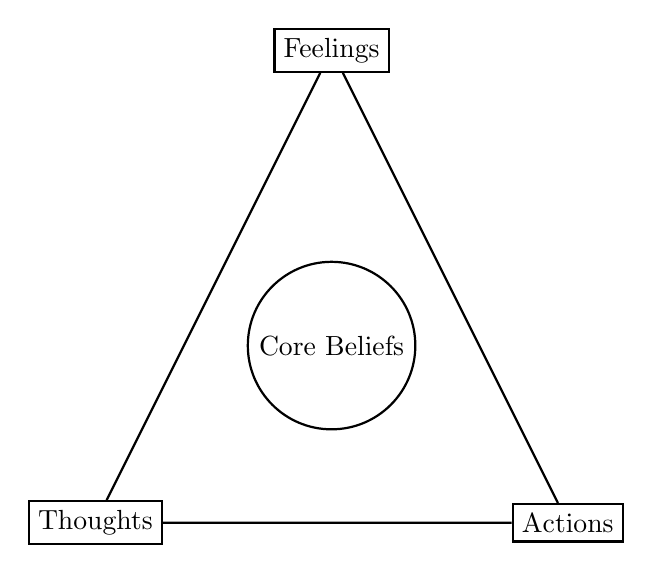
\begin{tikzpicture}
    \node[draw, thick] (A) at (0, 0) {Thoughts};
    \node[draw, thick] (B) at (6, 0) {Actions};
    \node[draw, thick] (C) at (3, 6) {Feelings};
    \node[draw, circle, thick] at (3, 2.25) {Core Beliefs}; 
    \draw[thick] (A) -- (B) -- (C) -- (A);
\end{tikzpicture}

\section{Main Questions Points from the Reading}

\begin{coloredlist}

    \item \textbf{Common Attributes of Cognitive Behavior Approaches:}
    \begin{coloredlist}
        \item Emphasis on the interaction between thoughts, feelings, and behaviors.
        \item Focus on identifying and modifying cognitive distortions or maladaptive thought patterns.
        \item Utilization of structured, goal-oriented, and present-focused interventions.
        \item Incorporation of self-monitoring and skills training to facilitate change.
    \end{coloredlist}

    \item \textbf{The ABC Model: Understanding Feelings, Thoughts, and Behavior:}
    \begin{coloredlist}
        \item \textbf{A (Activating Event):} The situation or trigger that initiates a reaction.
        \item \textbf{B (Beliefs):} The thoughts or interpretations about the event.
        \item \textbf{C (Consequences):} The emotional and behavioral responses resulting from the beliefs.
        \item This model helps individuals identify and alter irrational beliefs to change emotional and behavioral outcomes.
    \end{coloredlist}

    \item \textbf{Applying Cognitive Methods to Change Thinking and Behavior:}
    \begin{coloredlist}
        \item Use of cognitive restructuring to challenge and modify negative thoughts.
        \item Incorporation of behavioral experiments and exposure tasks to test and revise beliefs.
        \item Development of problem-solving and coping strategies.
        \item Implementation of self-monitoring techniques to increase awareness of thought patterns.
    \end{coloredlist}

    \item \textbf{Application of REBT in School Counseling:}
    \begin{coloredlist}
        \item Helping students identify and dispute irrational beliefs that lead to emotional distress.
        \item Teaching rational thinking to manage academic pressures and social challenges.
        \item Structuring interventions that promote adaptive coping and resilience.
    \end{coloredlist}

    \item \textbf{Aaron Beck's Unique Contributions to Cognitive Therapy:}
    \begin{coloredlist}
        \item Pioneering the development of cognitive therapy for depression.
        \item Introducing the concept of cognitive distortions and their role in emotional disorders.
        \item Establishing empirical methods for assessing and modifying dysfunctional thought patterns.
        \item Integrating cognitive techniques with behavioral interventions to enhance therapeutic outcomes.
    \end{coloredlist}

    \item \textbf{Basic Principles of Cognitive Therapy:}
    \begin{coloredlist}
        \item The idea that thoughts, rather than external events, determine feelings and behaviors.
        \item Identification and correction of cognitive distortions.
        \item Collaborative and active therapist-client relationship.
        \item Emphasis on skills acquisition and self-help strategies to promote long-term change.
    \end{coloredlist}

    \item \textbf{Application of the Cognitive Behavior Approach in School Counseling:}
    \begin{coloredlist}
        \item Addressing academic stress and performance anxiety.
        \item Enhancing students' problem-solving and coping skills.
        \item Promoting self-efficacy and adaptive thinking.
        \item Utilizing both individual and group counseling modalities.
    \end{coloredlist}

    \item \textbf{Basic Principles of Strengths-Based CBT:}
    \begin{coloredlist}
        \item Focus on identifying and leveraging individual strengths and resources.
        \item Emphasis on building resilience and fostering self-efficacy.
        \item Balancing recognition of challenges with the reinforcement of positive attributes.
        \item Collaborative goal-setting that empowers clients to capitalize on their strengths.
    \end{coloredlist}

    \item \textbf{Meichenbaum’s Three-Phase Process of Behavior Change:}
    \begin{coloredlist}
        \item \textbf{Conceptualization:} Understanding the problem through self-talk analysis.
        \item \textbf{Skill Acquisition:} Learning and practicing new coping and self-instructional strategies.
        \item \textbf{Application and Practice:} Implementing the acquired skills in real-life situations with reinforcement.
    \end{coloredlist}

    \item \textbf{Key Concepts and Phases of Meichenbaum’s Stress Inoculation Training:}
    \begin{coloredlist}
        \item \textbf{Conceptualization:} Identification of stressors and personal responses.
        \item \textbf{Skills Acquisition and Rehearsal:} Training in coping techniques and stress management.
        \item \textbf{Application and Follow-Through:} Practicing skills in both simulated and actual stressful situations.
    \end{coloredlist}

    \item \textbf{Strengths and Limitations of CBT from a Multicultural Perspective:}
    \begin{coloredlist}
        \item \textbf{Strengths:}
        \begin{coloredlist}
            \item Empirically supported, structured, and adaptable to diverse issues.
            \item Focus on empowerment and skill development.
        \end{coloredlist}
        \item \textbf{Limitations:}
        \begin{coloredlist}
            \item Potential to overlook cultural values and contextual factors.
            \item Need for adaptations to ensure cultural relevance and sensitivity.
        \end{coloredlist}
    \end{coloredlist}

    \item \textbf{Differentiating REBT from Cognitive Therapy Regarding Faulty Beliefs:}
    \begin{coloredlist}
        \item \textbf{REBT (Ellis):} Directly challenges and disputes irrational beliefs using a more confrontational and philosophical approach.
        \item \textbf{Cognitive Therapy (Beck):} Employs a collaborative approach to identify and modify cognitive distortions with structured interventions.
    \end{coloredlist}

    \item \textbf{Differences Among Ellis, Beck, Padesky, and Meichenbaum in CBT Practice:}
    \begin{coloredlist}
        \item \textbf{Ellis (REBT):} Emphasizes disputing irrational beliefs with a philosophical underpinning.
        \item \textbf{Beck:} Developed cognitive therapy focusing on depression and identifying cognitive distortions.
        \item \textbf{Padesky:} Advocates for collaborative empiricism and structured case formulation.
        \item \textbf{Meichenbaum:} Known for stress inoculation training and self-instructional methods.
    \end{coloredlist}
\end{coloredlist}
